%%%%%%%%%%%%%%%%%%%%%%%%%%%%%%%%%%%%%%%%%%%%%%%%%%%%%%%%%%%%%%%%%%%%%%%%%%%%%%%%
%2345678901234567890123456789012345678901234567890123456789012345678901234567890
%        1         2         3         4         5         6         7         8

\documentclass[letterpaper, 12 pt, Journal, onecolumn]{ieeeconf}  % Comment this line out if you need a4paper

%\documentclass[a4paper, 12pt, conference,onecolumn]{ieeeconf}      % Use this line for a4 paper
%\usepackage[utf8]{inputenc}
%\usepackage[english]{babel}

%\usepackage{amsthm}
\usepackage{float}
\usepackage{amsmath,amssymb,amsfonts}
%\usepackage{amsmath,amssymb}
%\theoremstyle{definition}
\newtheorem{remark}{Remark}
\newtheorem{definition}{Definition}
\usepackage[dvips]{color}
%\usepackage[a4paper]{geometry}
%\usepackage{epsfig}
\usepackage{subfigure}
\usepackage{soul}
\usepackage{multicol}
\usepackage{flushend}
\usepackage{color}
\usepackage{graphicx}      % include this line if your document contains figures
%\usepackage{natbib}        % required for bibliography
\usepackage{pgf}
%\usepackage{subcaption}                                   % Needed to meet printer requirements.
% See the \addtolength command later in the file to balance the column lengths
% on the last page of the document
\restylefloat{table}
\renewcommand{\baselinestretch}{1.25}
\title{\Large \bf
	Estimation of Delay in Time Series Using ARX Model Fitting
}

\author{\begin{tabular}{c}
		Linjian Xiang and Qing Zhao\\
		Department of Electrical and Computer Engineering \\
		Univ. of Alberta, Edmonton, Alberta, Canada\\
		\textbf{Date: June 19, 2018}
	\end{tabular}
}
\begin{document}
	\maketitle
	\thispagestyle{empty}
	\pagestyle{empty}
The objective of this report is to introduce a method for calculating the time-delays between time series that have dynamic relations. In a large-scale complex process, the dynamics among different time series are usually too complicated for the commonly used correlation-based time-delay estimation (TDE) to work well. For this reason, we investigate the Auto-Regression eXogenous (ARX) model identification based TDE method. In this approach, the delay between two time series is specifically modelled, the dynamic relation among the time series and their past histories are represented in a form of linear regression, and the best time-delay is found based on the estimated model. Additionally the model order is also determined. The order and delay together can be used to choose an appropriate value for the total delay shifts (i.e. the $h$ value), an important tuning parameter in the DPCA algorithm.\\

\section{Notations and Problem Formulations}

For convenience, we introduce the \textit{forward shift operator} $q$ by
\begin{equation}
qu(k) = u(k+1)
\end{equation}
and the \textit{backward shift operator} $q^{-1}$
\begin{equation}
q^{-1}u(k) = u(k-1)
\end{equation}
Assuming that there exists a time delay of $d$ steps between two time-series $u(k)$ and $y(k)$ which is introduced by the dynamic process, hence $u(k)$ and $y(k)$ are not only correlated but also have auto-correlations. Then the system equation relating the sequence $u(k)$ to the sequence $y(k)$ is
$$y(k)=g(k-d)\ast u(k)=\sum\limits_{i=0}^{n-1} g(i-d)u(k-i)$$
The above equation is the discrete-time convolution sum between the delayed $g(k)$, the (unknown) characteristic response of the system, and the input sequence $u(k)$. $d$ is the total number of delays. It can be written as
\begin{equation}
y(k) = \sum\limits_{i=0}^{n-1} g(i)q^{-d}q^{-i}u(k) = \left[\sum\limits_{i=0}^{n-1}g(i)q^{-i}\right]q^{-d}u(k) =G(q)u(k-d)
\end{equation}
by migrating the delay into the sequence $u(k)$, $G(q) =\sum\limits_{i=0}^{n-1}g(i)q^{-i}$ represents the delay-free linear time-invariant model with unknown order and parameters. In this report, using the model (3), an explicit model identification method is introduced for time-delay estimation (TDE). 
This method is tested on various data sets, the results are included and discussed in the report.

\section{ARX model based method}
	\subsection{Delay estimation}
Given model (3), note that $G(q)$ can also be represented in a fractional form 
$$ G(q)=\frac{B(q)}{A(q)},$$
where $A(q)$ and $B(q)$ are $n$th order and $m$th order polynomial, respectively, and $m\le n$, 
$$A(q)= 1+\sum\limits_{i=1}^n a_iq^{-i}, ~~B(q) = b_0+\sum\limits_{j=1}^m b_jq^{-j}$$
$a_i$ ($i=1,2,\dots,n$) and $b_j$ ($j=1,2,\dots,m$) are the unknown parameters, then we have 
$$
A(q)y(k)=B(q)u(k-d)
$$
By considering noises in the equation, the general ARX model (with delay) can be written as follows
\begin{equation} \label{eq:ARX}
	A(q)y(k)=B(q)u(k-d)+e(k)
\end{equation}
where $e(k)$ is the Gaussian white noise.

%If we incorporate and highlight the unknown parameter vector %$\theta$, the model becomes 
%$$y(k) = G(q,\theta)u(k)+H(q,\theta)e(k)$$
%$$H^{-1}(q,\theta)y(k) = H^{-1}(q,\theta)G(q,\theta)u(k)+e(k)$$
%Add $y(k)$ on both side
%$$y(k) = H^{-1}(q,\theta)G(q,\theta)u(k)+y(k)-H^{-1}(q,\theta)y(k)+e(k)$$
%$$= H^{-1}(q,\theta)G(q,\theta)u(k)+(\sum\limits_{k=1}^M %h(k)q^{-k})y(k)+e(k)$$
%Then the one-step-ahead prediction equation can be written as 
%\begin{equation} \label{eq:one_step_pre}
%	\tilde{y}(k|\theta) = H^{-1}(q,\theta)G(q,\theta)u(k)+(1-H^{-1}(q,\theta))y(k)
%\end{equation}
%	\subsection{Auto Regressive model}
%\

By substituting $A(q)$ and $B(q)$ in, the ARX model can be expressed by
\begin{equation}\label{eq:ARX_reformat}
y(k)+a_1y(k-1)+\ldots+a_ny(k-n)=b_0u(k-d)+\ldots+b_mu(k-m-d)+e(k)
\end{equation}
	
The prediction form of the above model with the unknown delay $d$ can be given as
\begin{equation} \label{eq:ARX_prediction}
\begin{aligned}
	\hat{y}(k,d) = b_0u(k-d)+b_1u(k-1-d) \ldots+b_mu(k-m-d)\\
	-a_1y(k-1)+\ldots+a_ny(k-n)
\end{aligned}
\end{equation}
now we define the regressor matrix and the parameter vector  
$$\phi(k,d) = [-y(k-1) \ldots -y(k-n) \enspace u(k-d) \ldots u(k-m-d)]^T$$ 
$$\theta=[a_1~\ldots ~a_n~b_0~\ldots~b_m]^T$$
Then the equation (~\ref{eq:ARX_reformat}) can be rewritten as
\begin{equation}
\hat{y}(k,d) = \theta^T \phi(k,d) = \phi^T(k,d)\theta
\end{equation}
	The unknown parameter $\theta$ can be estimated by Least-squares Estimation (LSE) directly. Then by iterating over $d$, the output error cost for each $d$ can be calculated. At last the best delay estimate $T_d$ is chosen with lowest output error cost, i.e.
\begin{equation}
T_d = arg~_{d} ~\biggl\{min ~\{[y(k)-\hat{y}(k,d)]^T[y(k)-\hat{y}(k,d)]\}\biggr\}
\end{equation}

	\subsection{Order Selection}
	In the above, usually $m$ and $n$ ($m\le n$) are unknown, and also need to be determined based on data. For simplicity, we assume $m=n$ so that only the model order $n$ needs to be decided. 
The \emph{Akaike Information Criterion} (AIC) is used for model order selection. The AIC is considered to be a measure for the relative quality of the model for a given dataset. The AIC value of the model can be written as:
	\begin{equation} \label{eq:AIC_eqn}
	 AIC = 2\mathbf{k} - 2\ln \mathbf{L}
	\end{equation}
Where $\mathbf{k}$ is the number of estimated parameters in the model and the $\mathbf{L}$ is the maximum value of the likelihood function for the model. The log-likelihood term $- 2log \mathbf{L}$ is called the \textit{goodness-of-fit} term, the larger \textit{goodness-of-fit} the better AIC. On the other hand, the AIC also includes the penalty term $2\mathbf{k}$ for the number of parameters, called bias correction, which is used to avoid model over-fitting.\\

The log-likelihood function for $N$ number of values in data set is \cite{AIC},
	\begin{equation} \label{eq:norm_distr}
	\ln \mathbf{L}(\mu,\sigma^2) = -\frac{N}{2}\ln(2\pi)-\frac{N}{2}\ln(\sigma^2)-\frac{1}{2\sigma^2}\sum_{i=1}^{N} (x_i-\mu)^2	
	\end{equation}
where $\mu$ and $\sigma$ are the mean and standard deviation, respectively.
We substitute the equation (\ref{eq:norm_distr}) and the numerically calculated standard deviation $\displaystyle{\frac{\sum_{i=1}^{N} (x_i-\mu)^2}{N}}$ into (\ref{eq:AIC_eqn}), then AIC becomes
	\begin{equation}
	AIC = 2\mathbf{k} + N \ln(\frac{\sum_{i=1}^{N} (x_i-\mu)^2}{N}) + N(\ln(2\pi)+1) 
	\end{equation}
For sets of candidate model orders, the preferred order $n$ is chosen as the one with the minimum AIC value.

\section{Delay estimation for DPCA parameter tuning}

In our project with Honeywell Process Solutions (HPS), it is proposed to use dynamic PCA (DPCA) and dynamic IPLS (DIPLS) for monitoring an industrial process. Details can be found from the previous Engage Grant report \cite{EGreport}. In a dynamic process, variables are time correlated. This means the value of each process variables at current time is dependent on the past histories of itself or other variables. To incorporate this feature, in DPCA an augmented step is added to form the augmented matrix $\bar{X}_i$ ($i$ being the \textit{i}th data point) from the original $X_i$ as $\bar{X}_{i}=[X_{i}^{T} \ X_{i-\tau}^{T}\ ... \ X_{i-(h-1)\tau}^{T} ]$. $\tau$ is the unit interval allowing for scaling in time for the augmented matrix. It is usually chosen as $\tau=1$, as we can see from commonly used difference equation, the unit step for differencing is 1, e.g. in equation (\ref{eq:ARX_reformat}). The parameter $h$ is total number of sample lags (shifts). In another word, the $h$ parameter determines the number of shifting action for generating the augmented $\bar{X}$ matrix. By using the ARX method described above, the total number of shifts $h$ can be determined by the order and the delay estimate in Section II. If we compare the form of $\bar{X}$ and the regressor matrix $\phi(k,d)$, it is noted that $h$ can be chosen as the maximum number of delay shifts in the regressor, which is $\max \{n,~m+d\}$. Because we assume $m=n$ for simplicity, then we choose $h=n+T_d$, the sum of the order and estimate of the delay.


\section{Testing Result}
The TDE method is tested on the simulated CSTR and Tennessee Eastman model(TE) data. For example, the CSTR model has 3 output variables and 2 input variables. The TDE method is applied on 1000 samples of CSTR data and the ARX fitted curve is shown as figure (\ref{fig:ARX_fitting}). 
\begin{figure}

	\begin{center}
	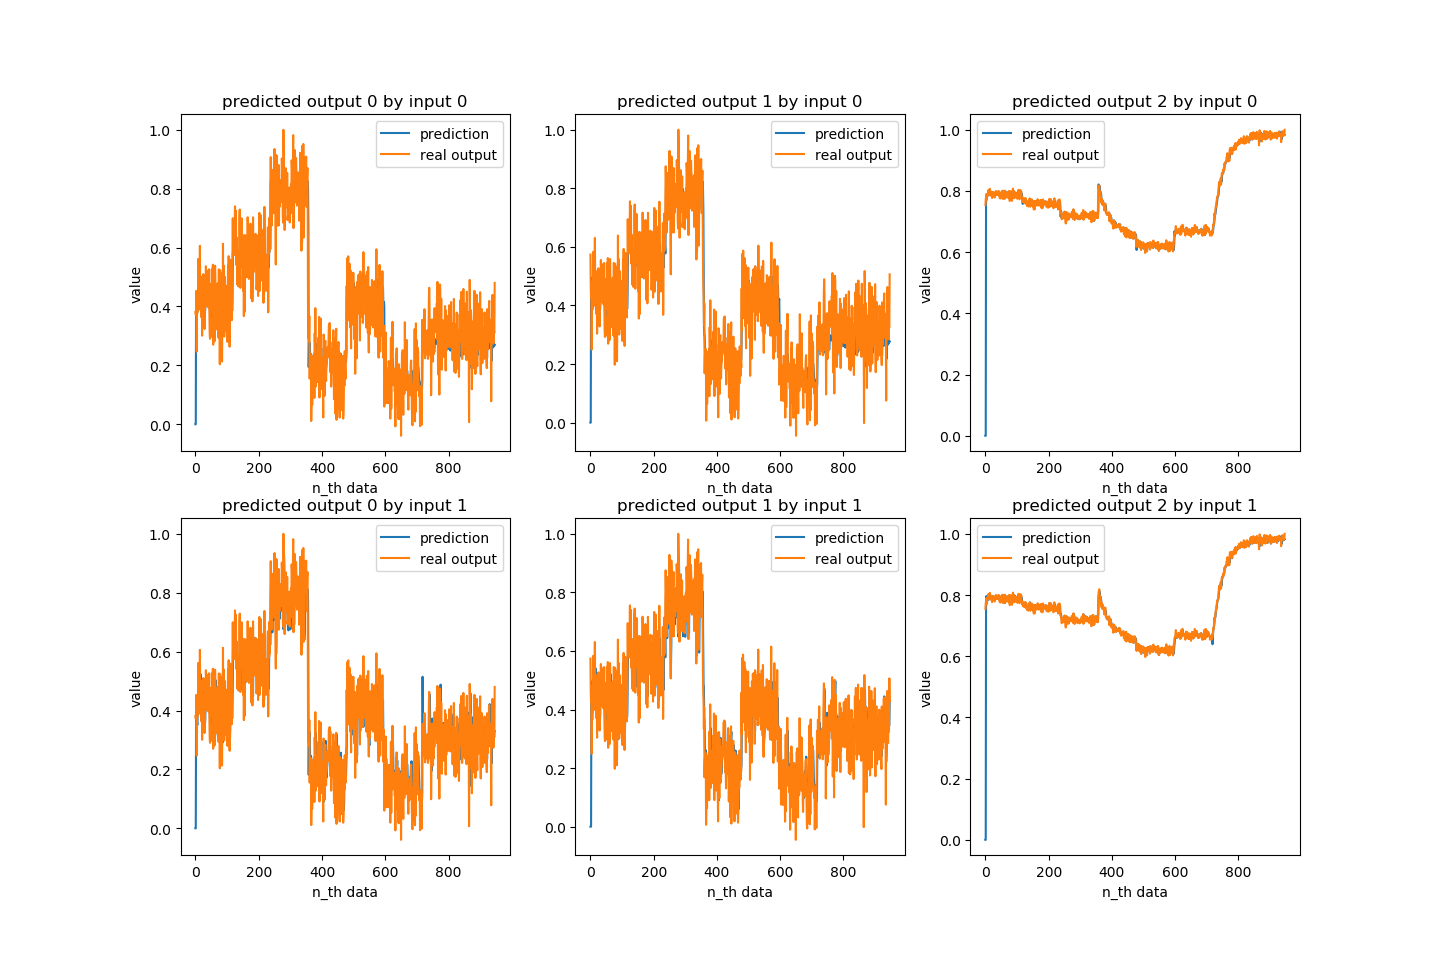
\includegraphics[scale=0.5]{cstr_arx_fit.png}
	\caption{ARX curve fitting}
	\label{fig:ARX_fitting}
	\end{center}
\end{figure}
For this data set delay we got is 1, the order is 2 and the suggested $h$ for DPCA is 3.


To certify the $h$ calculated by TDE works for DPCA, we firstly applied the DPCA on non-faulted data. Then insert numbers of fault into the system model and apply DPCA on model data. At last, the $T^2 Hotteling$ method is used to identify faults. 


The data from TE stripper is used for testing, the TE process manipulated variables $XMV(4)$ and $XMV(8)$ are used for TDE inputs and the TE process measurements $XMEAS(15)$ to $XMEAS(19)$ are used for TDE outputs. The fault detection between the $h$ calculated by ARX TDE method and the $RR-13$\cite{RR13} method are compared and shown as figure (\ref{fig:h_2}) and figure (\ref{fig:h_ARX}).  The $h$ computed by ARX method is $19$ and the $h$ calculated by $RR-13$ is 2.
\begin{figure}
	\begin{center}
	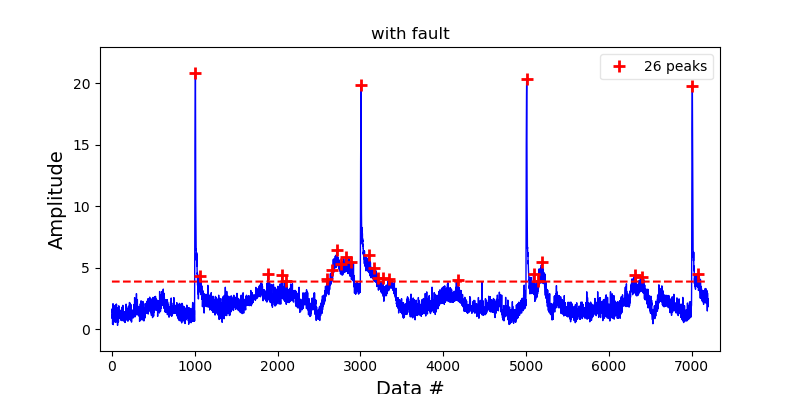
\includegraphics[scale=0.5]{2h_T2.png}
	\caption{h calculated by original method, h=2}
	\label{fig:h_2}
	\end{center}
\end{figure}

\begin{figure}
	\begin{center}
	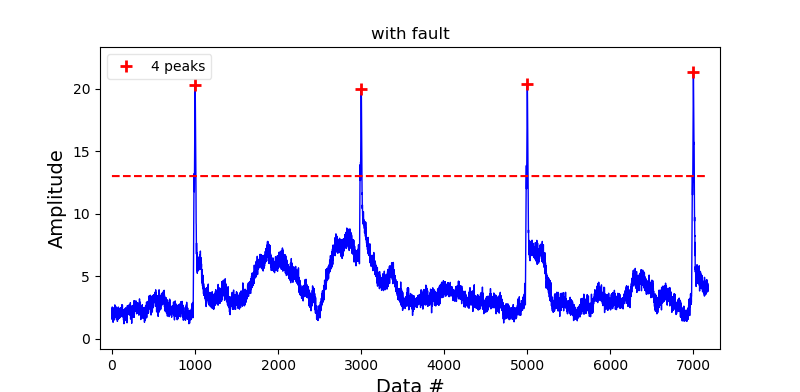
\includegraphics[scale=0.5]{ARX_TDE.png}
	\caption{h calculated by ARX method, h=19}
	\end{center}
	\label{fig:h_ARX}
\end{figure}

There are four faults added into the simulation, and the $T^2 Hotteling$ method were applied on these two simulation data sets. From the figures, it is clear to say that the $h$ calculated by ARX TDE method has better performance.

\begin{thebibliography}{9}
	
\bibitem{AIC} M. Lovric (ed.), International Encyclopedia of Statistical Science, DOI 10.1007/978-3-642-04898-2, Springer-Verlag, Berlin, Heidelberg, 2011

\bibitem{EGreport} B. Rashidi and Q. Zhao, ``Progress Report for Phase 1", the Engage Grant Project with HPS, Sept. 2, 2016, Univ. of Alberta.

\bibitem{RR13} T.J. Rato, M.S. Reis, Defining the structure of DPCA models and its impact on
process monitoring and prediction activities, Chemom. Intell. Lab. Syst. 125 (2013)
74–86, http://dx.doi.org/10.1016/j.chemolab.2013.03.009.
\end{thebibliography}


\end{document}
